\documentclass[11pt,a4paper]{article}

% Packages
\usepackage[utf8]{inputenc}
\usepackage[spanish, es-tabla]{babel}
\usepackage{caption}
\usepackage{listings}
\usepackage{adjustbox}
\usepackage{enumitem}
\usepackage{boldline}
\usepackage{amssymb, amsmath}
\usepackage[margin=1in]{geometry}
\usepackage{xcolor}
\usepackage{soul}
\usepackage{graphicx,wrapfig,lipsum}
\usepackage[bottom]{footmisc}
\usepackage{amsthm}
\usepackage{listings}
\usepackage[hidelinks]{hyperref} 
\usepackage{enumitem}% http://ctan.org/pkg/enumitem
\usepackage{algorithm}% http://ctan.org/pkg/algorithms
\usepackage{algpseudocode}% http://ctan.org/pkg/algorithmicx
\newcommand{\var}[1]{{\ttfamily#1}}% variable


% Meta
\title{Título}
\author{Pedro Bonilla Nadal\\Ana Peña Arnedo}
\date{\today}

% Custom
\providecommand{\abs}[1]{\lvert#1\rvert}
\setlength\parindent{0pt}
\definecolor{Light}{gray}{.90}
\newcommand\ddfrac[2]{\frac{\displaystyle #1}{\displaystyle #2}}

\begin{document}
\begin{titlepage}
  \centering
  
  \vspace{10cm}
  
\includegraphics[width=0.6\textwidth]{images/portada.png}\par\vspace{1cm}
  {\scshape\large Fundamentos de Redes \par} \vspace{1cm}
  \vspace{0.4cm}
  {\large\itshape Memoria de la exposición\\}
  \vspace{0.6cm}
  {\large\itshape  Pedro Bonilla Nadal\\Ana Peña Arnedo \par} \vspace{1.00cm}

  \vfill
  % Bottom of the page
  {\large \today\par}

\end{titlepage}
\begin{center}
	
\includegraphics[scale=.42]{images/logo.png}
\end{center}


\section{Introducción}
Hoy en día, la información es todo. Las grandes compañias de internet han alcanzado un modelo  de negocio en el cual no tienen que exigirte dinero para conseguir beneficios. Estos te cobran por una aceptación de ceder tu información para traficar con ella. \\

En la actualidad, con el objetivo de mantener un sistema de comercio que no tenga que ser mantenido por un organismo que, por lo tanto mantenga poder sobre sus usuarios. Este tipo de comercio 'tradicional' \ incluye organizaciones como, por ejemplo, amazon, que facilita la compra-venta respaldada por una compañía, o los bancos centrales, los cuales mantienen las divisas y son los responsables del cuidado y mantención de la divisa. Como sabemos que una compañia esté al cargo del cuidado del sistema, (es decir, que tenga un sistema centralizado) tiene una serie de beneficios e inconvenientes. \\

Por un lado el sistema centralizado con control por una compañía, como la contratación de especialistas para almacenar y proteger la seguridad, y reduce los tiempos de almacenamiento y actualización del sistema. \\

Por otro lado, donde hay una ventaja, hay un inconveniente. Como se ha podido ver en alguna ocasion\footnotemark esta organización habilita a grandes compañías y estados a filtrar, robar o modificar a información sensible  de los usuarios. Esta vulnerabilidad ha llegado a ser calificada como el 'pecado original'\ de internet, pues este siempre intento ser una plataforma de caracter descentralizado.\\

	Satoshi Nakamoto inció en 2008 el desarrollo de bitcoin. Este hecho desencadenaria un desarrollo increible en el area de las divisas con centralizadas, es decir un sistema monetario que no necesitase de un sistema bancario o de un valor predeterminado. También sorprendió mucho a la comunidad la aplicación de la tecnología de la cadena de bloques, como una herramienta basada en la distribución del conseno. A raiz de estas surgieron otras teconologías basadas en la cadena de bloques, como namecoin, añadiendo. Lo que ethereum pretende es proveer una cadena de bloques con un leguanje turing completo integrado que pueda ser usado para el desarrollo de contratos inteligentes, permitiendo a los usarios la ceanción de proyectos solo escribiendo la logica de estos en unas pocas lineas de código. Algunos de estos poryectos, sacados del la propia web \url{ethereum.org} serían la creación de un crowdfounding que no sea basado en la confianza si no en un contrato que almacenará el dinero de los contribuyentes, una organización autónoma democrática.\\

\footnotetext{\url{https://www.theguardian.com/world/2013/jun/06/nsa-phone-records-verizon-court-order}}

En resumen, nuestra moneda lo que intenta es crear un 'ordenador  global' que descentralice el actual cliente-servidor. Con Ethereum en lugar de tener un servidor tendríamos un conjunto de nodos, almacenados por voluntarios alrededor del mundo . Sobre este sistema, la comunidad podrá competir por ofrecer servicios, además de consumirlos.


Ejemplifiquemos la diferencia: navegar por una app-store cualquiera nos ofrecerá una serie de aplicaciones en las cuales contactaremos con un servidor que nos proverá del servicio, generalmente gestionado por un tercero no relacionado (de manera directa) con la transacción.\\

Ethereum, si todo funciona, devolvería la propiedad de la información a su dueño, de modo que solo el usuario puede modificar la información, y no ninguna entidad externa.\\



\section{Ethereum\\}


\subsection{Historia.}
	En 2012, un joven de 19 años propuso una nueva plataforma, con el objetivo de trasnfomar por entero internet. Vitalik Buterin, un programador de Toronto empezó su investigación en la cadena de bloques en 2011. Co-fundó el portal web Bitcoin Magazine y trabajó para compañías de la materia. En el camino pensó en una plataforma que fuera más allá de las posibilidades del bitcoin.\\
	
	Con esta idea nació ethereum, una plataforma para la creación de contratos inteligentes (smart contract). Después de publicar en 2014 el white paper, otros desarrolladores se unieron al proyecto. \\

	Para lanzar el poryecto se inició un crowdfounding en julio de 2014, donde los participantes compraban \hyperref[sec:ether]{\textbf{\underline{ether}}} . Después de reunir más de 18 millones de dolares, se inició y en 2015 se lanzó una plataforma, no demasiado user-friendly, pero con comandos el linea que permitía la creación de aplicaciones descentralizadas.\\

Este nuevo tipo de contratos caló entre el público llamando la atención de gigantes tecnológicos como IBM y gran cantidad de desarrolladores. El dinero recaudado inicialmente está gestionado por Etherum foundaion\footnotemark, una compañía sin animo de lucro ubicada en Suiza.	\\

\footnotetext{\url{https://www.ethereum.org/foundation}}

\subsubsection{Hardfork y el cisma de ethereum}
\begin{wrapfigure}{r}{5.5cm}
\caption{\ \ }

\includegraphics[width=5.5cm]{images/classic1.png}
\end{wrapfigure} 
%------------------------------------------
En 2016 una organización autonoma descentralizada llamada The DAO, un conjunto de contratos inteligentes reunieron un total de USD \$150 millones en una crowdsale. Al final DAO esplotó cuando en junio USD \$50 millones en Ether fueron reclamados de manera anonima. El suceso inició un debate sobre si de debía hacer un 
\hyperref[sec:hardfork]{\textbf{\underline{hardfork}}} y como resutado de la disputa, la red se dividió en dos: Ethereum, el objetivo de este trabajo,que continuó la cadena modificada, y Ethereum Classic, que continuó la cadena original. Desde entonces se generó un conflicto entre ambas comunidades.\\


\subsection{Funcionamiento.\\} 
Una vez sabemos lo que es ethereum, profundizamos en el funcionamiento de la plataforma.
Al usar ethereum, la ‘app’ no requiere ninguna entidad para almacenar y controlar sus datos. Para conseguirlo, ethereum hace uso del protocolo de bitcoin y su diseño de la cadena de bloques, aunque lo ajusta de manera que puede respaldar aplicaciones además del dinero. Sin embargo, ethereum persigue abstraerse del diseño de bitcoin con el fin de que los desaprobadores puedan crear aplicaciones o acuerdos que incluyan medidas adicionales, nuevas normas de propiedad, formatos alternativos de transacciones o diferentes maneras de transferir estados.\\

El objetivo del lenguaje de programación ‘Turing-completo’ de ethereum es permitir a los
desarrolladores escribir más programas (que los que permite la linea de comandos de bitcoin) en los que las transacciones en la cadena de bloques puedan gobernar y automatizar resultados específicos. Tengamos en cuenta que un lenguaj turing-completo es capaz de generar (en teoría) los mismos programas que son desarrollables c++. Esta flexibilidad que ofrece ethereum es  la innovacioń fundamental de ethereum sobre otras plataformas basadas en protocolo bitcoin.\\

\subsubsection{Bitcoin como sistema de transición de estados}

Desde un punto de vista técnico, el ledger de Bitcoin puede verse como un sistema de
transición de estados, donde hay un estado que consiste en el estado de propiedad de todos los bitcoins existentes además de una función de transición de estado que toma un estado y una transacción y genera un nuevo estado que es el resultado. De este modo obtendríamos un autómata, y además al haber un número finitio de bitcoin, podemos decir que es finito en teoría (aunque no en práctica, pues la cantidad de variaciones de la red es casi inabarcable).\\

 En un sistema bancario estándar, por ejemplo, el estado es una hoja de balance, una transacción es una petición para mover una determinada cantidad de dinero de “A” a “B”, y la función de transición de estado reduce esa cantidad de dinero en la cuenta de “A” y la incrementa en la cuenta de “B”. Si, en primer lugar, la cuenta de “A” tiene una cantidad menor a la indicada, la función de transición de estado devuelve un error. Por lo tanto, podría definirse formalmente:
\begin{lstlisting}

APPLY( S , TX ) -> S' o ERROR

\end{lstlisting}


En el sistema bancario definido arriba:
\begin{lstlisting}

APPLY( { Ana: 50 , Pedro: 50 } , "enviar 20 de Ana a Pedro" ) 
{ Ana: 30 , Pedro: 70 }

\end{lstlisting}
Sin embargo:
\begin{lstlisting}

APPLY( { Ana: 50 , Pedro: 50 } , "enviar 70 de Ana a Pedro" ) 
ERROR

\end{lstlisting}


El estado en Bitcoin es la colección de todas las monedas (técnicamente, “transacciones no
gastadas” o UTXO - “unspent transaction outputs”) que han sido creadas pero aún no se han
gastado, con cada UTXO que tiene una denominación y un propietario (definido por una dirección
de 20 bytes que es esencialmente una clave pública criptográfica). Una transacción contiene una
o más entradas, y cada entrada contiene una referencia a una UTXO existente y a una firma
criptográfica producida por la clave privada asociada con la dirección del propietario; y una o más
salidas, cada una de las cuales contiene una nueva UTXO para añadirla al estado.
La función de transición de estado APPLY( S , TX ) $->$S' puede definirse aproximadamente
como sigue:
\begin{enumerate}
\item Para cada entrada en TX:
i. Si la UTXO referenciada no está en S, devuelve un error.
ii. Si la firma proporcionada no concuerda con el propietario de la UTXO, devuelve
un error.
\item Si el conjunto de denominaciones de toda entrada UTXO es menor que el conjunto de
denominaciones de toda salida UTXO, devuelve un error.
\item Devuelve S con toda entrada UTXO eliminada y toda salida UTXO añadida.
La primera mitad del primer paso evita que los que envían transacciones gasten monedas que no
\end{enumerate}
existen, la segunda mitad del primer paso evita que los que envían transacciones gasten las
monedas de otras personas, y el segundo paso impone la conservación del valor. A la hora de
usar esto para pagos, el protocolo es como sigue. Supongamos que Ana quiere enviar 11.7 BTC a
Pedro. Primero, Ana buscará un conjunto de UTXO disponibles que ella posea que sume un total
de al menos 11.7 BTC. Realmente, Ana no será capaz de obtener exactamente 11.7 BTC;
digamos que lo menos que puede obtener es 6+4+2=12. Entonces ella creará una transacción con
esas tres entradas y dos salidas. La primera salida será 11.7 BTC con la dirección de Pedro como
su propietario, y la segunda salida serán los restantes 0.3 BTC de “cambio”, siendo su propietaria
la propia Ana.

\subsubsection{Cadena de Bloques de Ethereum}
La estructura de la cadena de bloques de ethereum es muy similar a la de bitcoin, dado que se trata de un registro compartido de la historia de transacciones completa. Cada nodo en la red almacena una copia de este historial.\\

La gran diferencia con ethereum es que sus nodos almacenan también el estado más reciente de cada contrato inteligente, además de todas las transacciones de ether.
Para cada aplicación de ethereum, la red tiene que mantener un seguimiento del ‘estado’ o
información actual de todas estas aplicaciones, incluyendo el saldo de cada usuario, todo el código del contrato inteligente y dónde se almacena todo. Bitcoin usa salidas de transacción no utilizadas para rastrear quién tiene cuánto bitcoin.
 Aunque suena complejo, la idea es bastante simple. Cada vez que se hace una transacción de
bitcoin, la red ‘rompe’ la cantidad total como si fuera dinero impreso, emitiendo bitcoins de vuelta de una forma que hace que la información manejada se comporte como las monedas o cambio físico.\\

Para efectuar futuras transacciones, la red de bitcoin tiene que añadir todas las piezas de cambio, que se clasifican en ‘gastadas’ o ‘no gastadas’. Ethereum, por otro lado, utiliza cuentas. Como en fondos de cuentas bancarias, las ‘fichas’ de ether aparecen en una cartera, y pueden ser portados (por así decirlo) a otra cuenta. Los fondos siempre están en algún sitio, pero no tienen lo que podría llamarse una relación continua. 


\textcolor{red}{Extender}. 

\subsubsection{Máquina Virtual de Ethereum}
Con ethereum, cada vez que se usa un programa, una red de miles de computadores lo procesa. Los contratos escritos en un lenguaje de programación específico de contrato inteligente se compilan en ‘bytecode’, lo que una prestación llamada ‘ethereum virtual machine’ (EVM) puede leer y ejecutar. Todos los nodos ejecutan este contrato usando sus EVMs.  Cada vez que un usuario realiza alguna acción, todos los nodos de la red tienen que estar de acuerdo en que ese cambio se ha efectuado.
El objetivo aquí es que la red de mineros y nodos tomen la responsabilidad de transferir el cambio de estado a estado, en lugar de cualquier autoridad como PayPal o un banco. Los mineros de bitcoin validan el cambio de propiedad de bitcoins de una persona a otra. La EVM ejecuta un  contrato con las reglas que el desarrollador programó inicialmente. \\

El cálculo real en la EVM se consigue mediante un lenguaje ‘bytecode’ basado en pilas, pero los desarrolladores pueden escribir contratos inteligentes en lenguajes de alto nivel como Solidity o Serpent, más fáciles de leer y escribir para las personas, dado que bytecode es un lenguaje poco legible, pero mmás interpretable a un ordenador, análogo al lenguaje máquina. Los mineros son los que evitan un mal comportamiento. A diferencia de en bitcoin, la cantidad de nodos es escalable, por lo que la ausencia de mineros no será un problema a largo plazo. Por ejemplo, deben asegurarse de que
nadie gasta dinero más de una vez, y rechazar contratos inteligentes que no se han pagado. Existen varios miles de nodos de ethereum ahí fuera, y cada uno de ellos está compilando y ejecutando el mismo código.\\

Podemos pensar que todo esto tiene un coste mucho mayor al de cálculos ordinarios, lo cual es cierto. Por ello la red solo debe usarse para casos de uso particular. El tutorial oficial de desarrollo de ethereum reconoce esta ineficacia, declarando:
"A grandes rasgos, una buena heurística para usar es que no podrás hacer nada en la EVM que no puedas hacer en un teléfono inteligente de 1999".\\

Este lenguaje será fundamental para la implementación de los contratos inteligentes o samrt contract, pues es lo que permite generar los entes de funcionamiento autonómo para el desarrollo de estos.

\subsubsection{mensajes, transacciones y estado de transición de ethereum}

Los mensajes en ethereum son parecidos de cierto modo a las transacciones de en otros  sistemas de cadena de bloques, pero  con algunas caracteristicas llamativas. Un mensaje puede ser creado tanto por una entidad externa como por un contrato, los mensajes pueden contener datos o, si el mensaje es recibido por un contrato, este tiene la opcion de responder. Esto implica que un mensaje en etherum puede toar el aspecto de función.\\

El termino transacción es usado en  ethereum para referirse a un paquete firado que coniene un mensaje para ser enviado por una cuenta externa. Las transacciones serian el recipiente del mensaje, una firma identificando el remitente, la cantidad de ether que mandar, y además los dos valores importantes de Gasprice y Startgas.\\

Para prevenir el uso de bucles infinitos, cada transacción requiere marcar cuantos pasos de computación pueden ser realizados. Startgas es el límite, y Gasprice es lacuotaa pagar al minero por iteración. Si la transacción se queda sin "gas" todos los cambios de estado en la cadena se revierten. Si llega a un halts con algun gas restante, este se le envia al contratante. \\

Como veremos, es importante que una transacción tenga los mismos derecho que un usuario para el desarrollo conveniente de los contratos inteligentes, incluyendo la habilidad de mandar mensajes de unos a otros.\\


\subsubsection{Contratos inteligentes.}

Un contrato inteligente (en inglés Smart contract) es un programa informático que facilita, asegura, hace cumplir y ejecuta acuerdos registrados entre dos o más partes (por ejemplo personas u organizaciones). Como tales ellos les ayudarían en la negociación y definición de tales acuerdos que causarán que ciertas acciones sucedan como resultado de que se cumplan una serie de condiciones específicas.\\

Un contrato inteligente es un programa que vive en un sistema no controlado por ninguna de las partes, o sus agentes, y que ejecuta un contrato automático el cual funciona como una sentencia if de cualquier otro programa de ordenador. Con la diferencia de que se realiza de una manera que interactúa con activos reales. Cuando se dispara una condición pre-programada, no sujeta a ningún tipo de valoración humana, el contrato inteligente ejecuta la cláusula contractual correspondiente.\\

Tienen como objetivo brindar una seguridad superior a la ley de contrato tradicional y reducir costos de transacción asociados a la contratación. La transferencia de valor digital mediante un sistema que no requiere confianza abre la puerta a nuevas aplicaciones que pueden hacer uso de los contratos inteligentes, como es el caso de ethereum.\\

Bitcoin inició este proceso antes, pero su uso está limitado a el uso como divisa únicamente. Sin embargo, el lenguaje turing completo de ethereum que permite a los desarrolladores escribir sus propios programas, soporta que estos desarrollen sus propios contratos inteligentes, es decir, agentes que que controlen todo el proceso del negocio.\\

\begin{center}
	
	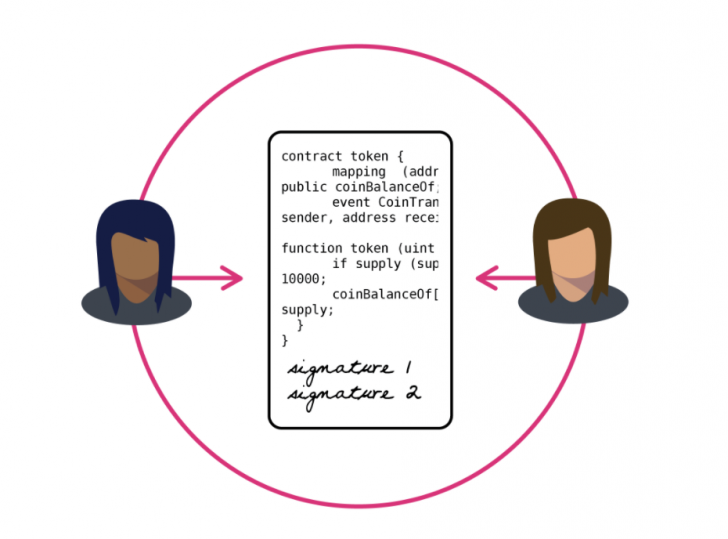
\includegraphics[scale=.45]{images/smart.png}
\end{center}

Estos agentes, no controlados por ninguna de las partes, son los que, (una vez aceptado el contrato) fuerzen a su cumplimiento o devuelvan una vez el contrato se ha terminado de forma fallida al estado original la cadena de bloques.\\


Un punto importante a considerar como fallo de los contratos inteligentes es que ambas partes han de tener acceso al código del smart contract, y comprender activamente (no porque se lo haya explicado alguien) que hace y porque lo hace el programa brindado. Si estas condiciones se cumplen, y ambas partes saben lo que están aceptando su cumplimiento es obligado, de modo que si no se cumpliera el contrato no tendría ningún efecto.\\

Los contratos inteligente pueden, entre otras muchas cosas:
\begin{itemize}
	\item Sevir como un programa de firma de comunidad, en el cual los fondos se invierten solo cuando hay una mayoría prefijada de personas que aceptan la inversión. Del mismo modo este contrato podría ser reformado en el código que lo constituye cuando la misma mayoría (por ejemplo, del 80\%) lo acpeta.
	\item Controlar acuerdos entre ususarios, por ejemplo, cuando uno contrata un seguro con el otro.
	\item Gestionar el funcionamiento de otros contratos (recordemos que en ethereum un contrato puede realizar las mismas acciones que un usuario).
\end{itemize}

Pongamos un  ejemplo de este último:\\

Cuando en una compañía una mayoría acepte bajar la temperatura del AC, otro contrato comproabría la previsión meteorológica para ver si está acción debe tener caracter permanente, y otro contactaría con la base de datos para enviar la información recogida en los anteriores a la base de datos.
transaction fees, which depend on the amount of computational power required.

\subsubsection{Minería}
\url{https://www.coindesk.com/information/ethereum-mining-works/}
\url{https://www.coindesk.com/information/how-to-mine-ethereum/}

\subsubsection{Hardfork}
\label{sec:hardfork}
\url{https://es.cointelegraph.com/news/hard-fork-y-soft-fork-en-qu\%C3\%A9-consisten-y-cu\%C3\%A1les-son-sus-diferencias}


\section {Aplicaciones.} 
En general, hay tres tipo de aplicaciones montadas encima de ethereum. La primera categoría es aplicaciones de financiación, las cuales habilitan una vía más amplia de gestionar los contratos. La segunda categoría son aplicaciones semifinancieras,donde el dinero está involucrado pero hay una gran parte de importancia en valores no monetarios. Por último estarían las plataformas para organizaciones de gobieron descentralizado y voto, no monetarias en ningún sentido.

\subsection{Sistemas de Token.}

Los sistemas de tokens basados en cande de bloques tienen multitud de aplicaciones, desde representar alguna divisa o materia relacionada con el mundo real como el precio del venta de oro o intercambio de USD. Otros usos serían tokens en relación a conceptos como propiedad intelectual o sistemas no relacionados en ningún punto, no financieros en ningún aspecto. \\

Los sistemas de token son muy fáciles de implementar con ethereum. El punto clave para entender el funcionamiento es darse cuenta de que cualquier sistema de token es, fundamentalmente, una base de datos con una operación: Quita $x$ unidades a $A$ y dáselas a $B$, con condición de que:
\begin{itemize}
	\item $A$ tiene al mmenos $X$ unidades antes de la transacción.
	\item La transacción está aprobada por $A$. 
\end{itemize}

Todo lo restante sería implementar esta lógica en un contrato. Un código básico sería:\\

    
\begin{algorithm}
  \caption{Contrato de Tokens.}\label{token}
  \begin{algorithmic}[1]
    \Procedure{Token}{$msg, contract$}			\Comment{msg contiene la información de la comunicación}\\ \Comment{contract contiene información del contrato}
    
    \State from = $msg$.sender
	\State to = $msg$.data[0]
	\State value = $msg$.data[1]
    \If{contract.storage[from] $>=$ value}
		\State contract.storage[from] = contract.storage[from] ­ value
		\State contract.storage[to] = contract.storage[to] + value
    \EndIf
    \EndProcedure
  \end{algorithmic}
\end{algorithm}

Esto sería una implementación en pseudo-código de la lógica básica del sistema bancario ya descrito.


\subsection{Sistema de comprobación de identidad}

INVESTIGAR Y DESARROLLAR

\subsection{Decentralized File Storage}

En el último tiempo han surgido..


\subsection{Decentralized Autonomous Organizations}
\label{sec:dao}

\section{Particularidades.}

\subsection{Ether.}
\label{sec:ether}

AQUÍ VA LA PAGINA QUE HAY QUE TRADUCIR.	\\
\url{https://www.coindesk.com/information/what-is-ether-ethereum-cryptocurrency/}	\\
si pinchas aquí te lleva.

\subsection{DoS attack.}
Dado el incidente del DAO, hemos de explicar en que consiste este ataque hecho a la red.		 \\
\url{https://en.wikipedia.org/wiki/Denial-of-service_attack}\\
Esto se solvento hipotéticamente a finales de 2016 al mejorar la denfensa en este tipo de ataques. \textcolor{red}{investigar como lo han hecho}

\subsection{Escalabilidad}
\subsection{Minería centralizada}

\newpage
\begin{center}
	
\includegraphics[scale=.42]{images/logo.png}
\end{center}

\tableofcontents
\end{document}